%%%%%%%%%%%%%%%%%%%%%%%%%%%%%%%%%%%%%%%%%
% Programming/Coding Assignment
% LaTeX Template
%
% This template has been downloaded from:
% http://www.latextemplates.com
%
% Original author:
% Ted Pavlic (http://www.tedpavlic.com)
%
% Note:
% The \lipsum[#] commands throughout this template generate dummy text
% to fill the template out. These commands should all be removed when 
% writing assignment content.
%
% This template uses a Perl script as an example snippet of code, most other
% languages are also usable. Configure them in the "CODE INCLUSION 
% CONFIGURATION" section.
%
%%%%%%%%%%%%%%%%%%%%%%%%%%%%%%%%%%%%%%%%%

%----------------------------------------------------------------------------------------
%	PACKAGES AND OTHER DOCUMENT CONFIGURATIONS
%----------------------------------------------------------------------------------------

\documentclass{article}

\usepackage{fancyhdr} % Required for custom headers
\usepackage{lastpage} % Required to determine the last page for the footer
\usepackage{extramarks} % Required for headers and footers
\usepackage[usenames,dvipsnames]{color} % Required for custom colors
\usepackage{graphicx} % Required to insert images
\usepackage{listings} % Required for insertion of code
\usepackage{courier} % Required for the courier font
\usepackage{lipsum} % Used for inserting dummy 'Lorem ipsum' text into the template
\usepackage{times}

% Margins
\topmargin=-0.45in
\evensidemargin=0in
\oddsidemargin=0in
\textwidth=6.5in
\textheight=9.0in
\headsep=0.25in

\linespread{1.1} % Line spacing

% Set up the header and footer
\pagestyle{fancy}
\lhead{\hmwkAuthorName} % Top left header
\chead{\hmwkClass\ (\hmwkClassInstructor\ \hmwkClassTime): \hmwkTitle} % Top center head
\rhead{\firstxmark} % Top right header
\lfoot{\lastxmark} % Bottom left footer
\cfoot{} % Bottom center footer
\rfoot{Page\ \thepage\ of\ \protect\pageref{LastPage}} % Bottom right footer
\renewcommand\headrulewidth{0.4pt} % Size of the header rule
\renewcommand\footrulewidth{0.4pt} % Size of the footer rule

\setlength\parindent{0pt} % Removes all indentation from paragraphs

%----------------------------------------------------------------------------------------
%	CODE INCLUSION CONFIGURATION
%----------------------------------------------------------------------------------------

\definecolor{MyDarkGreen}{rgb}{0.0,0.4,0.0} % This is the color used for comments
\lstloadlanguages{Perl} % Load Perl syntax for listings, for a list of other languages supported see: ftp://ftp.tex.ac.uk/tex-archive/macros/latex/contrib/listings/listings.pdf
\lstset{language=C, % Use Perl in this example
        frame=single, % Single frame around code
        basicstyle=\small\ttfamily, % Use small true type font
        keywordstyle=[1]\color{Blue}\bf, % Perl functions bold and blue
        keywordstyle=[2]\color{Purple}, % Perl function arguments purple
        keywordstyle=[3]\color{Blue}\underbar, % Custom functions underlined and blue
        identifierstyle=, % Nothing special about identifiers                                         
        commentstyle=\usefont{T1}{pcr}{m}{sl}\color{MyDarkGreen}\small, % Comments small dark green courier font
        stringstyle=\color{Purple}, % Strings are purple
        showstringspaces=false, % Don't put marks in string spaces
        tabsize=5, % 5 spaces per tab
        %
        % Put standard Perl functions not included in the default language here
        morekeywords={rand},
        %
        % Put Perl function parameters here
        morekeywords=[2]{on, off, interp},
        %
        % Put user defined functions here
        morekeywords=[3]{test},
       	%
        morecomment=[l][\color{Blue}]{...}, % Line continuation (...) like blue comment
        numbers=left, % Line numbers on left
        firstnumber=1, % Line numbers start with line 1
        numberstyle=\tiny\color{Blue}, % Line numbers are blue and small
        stepnumber=5 % Line numbers go in steps of 5
}

% Creates a new command to include a perl script, the first parameter is the filename of the script (without .pl), the second parameter is the caption
\newcommand{\code}[2]{
\begin{itemize}
\item[]\lstinputlisting[caption=#2,label=#1]{#1}
\end{itemize}
}

%----------------------------------------------------------------------------------------
%	DOCUMENT STRUCTURE COMMANDS
%	Skip this unless you know what you're doing
%----------------------------------------------------------------------------------------

% Header and footer for when a page split occurs within a problem environment
\newcommand{\enterProblemHeader}[1]{
\nobreak\extramarks{#1}{#1 continued on next page\ldots}\nobreak
\nobreak\extramarks{#1 (continued)}{#1 continued on next page\ldots}\nobreak
}

% Header and footer for when a page split occurs between problem environments
\newcommand{\exitProblemHeader}[1]{
\nobreak\extramarks{#1 (continued)}{#1 continued on next page\ldots}\nobreak
\nobreak\extramarks{#1}{}\nobreak
}

\setcounter{secnumdepth}{0} % Removes default section numbers
\newcounter{homeworkProblemCounter} % Creates a counter to keep track of the number of problems

\newcommand{\homeworkProblemName}{}
\newenvironment{homeworkProblem}[1][Problem \arabic{homeworkProblemCounter}]{ % Makes a new environment called homeworkProblem which takes 1 argument (custom name) but the default is "Problem #"
\stepcounter{homeworkProblemCounter} % Increase counter for number of problems
\renewcommand{\homeworkProblemName}{#1} % Assign \homeworkProblemName the name of the problem
\section{\homeworkProblemName} % Make a section in the document with the custom problem count
\enterProblemHeader{\homeworkProblemName} % Header and footer within the environment
}{
\exitProblemHeader{\homeworkProblemName} % Header and footer after the environment
}

\newcommand{\problemAnswer}[1]{ % Defines the problem answer command with the content as the only argument
\noindent\framebox[\columnwidth][c]{\begin{minipage}{0.98\columnwidth}#1\end{minipage}} % Makes the box around the problem answer and puts the content inside
}

\newcommand{\homeworkSectionName}{}
\newenvironment{homeworkSection}[1]{ % New environment for sections within homework problems, takes 1 argument - the name of the section
\renewcommand{\homeworkSectionName}{#1} % Assign \homeworkSectionName to the name of the section from the environment argument
\subsection{\homeworkSectionName} % Make a subsection with the custom name of the subsection
\enterProblemHeader{\homeworkProblemName\ [\homeworkSectionName]} % Header and footer within the environment
}{
\enterProblemHeader{\homeworkProblemName} % Header and footer after the environment
}

%----------------------------------------------------------------------------------------
%	NAME AND CLASS SECTION
%----------------------------------------------------------------------------------------

\newcommand{\hmwkTitle}{Expression Parser Assignment} % Assignment title
\newcommand{\hmwkDueDate}{Monday,\ March\ 24,\ 2014} % Due date
\newcommand{\hmwkClass}{CMPSCI\ 230} % Course/class
\newcommand{\hmwkClassTime}{1:00pm} % Class/lecture time
\newcommand{\hmwkClassInstructor}{Tim Richards} % Teacher/lecturer
\newcommand{\hmwkAuthorName}{Tim Richards} % Your name

%----------------------------------------------------------------------------------------
%	TITLE PAGE
%----------------------------------------------------------------------------------------

\title{
\vspace{2in}
\textmd{\textbf{\hmwkClass:\ \hmwkTitle}}\\
\normalsize\vspace{0.1in}\small{Due\ on\ \hmwkDueDate}\\
\vspace{0.1in}\large{\textit{\hmwkClassInstructor\ \hmwkClassTime}}
\vspace{3in}
}

\author{\textbf{\hmwkAuthorName}}
\date{} % Insert date here if you want it to appear below your name

%----------------------------------------------------------------------------------------

\begin{document}

\maketitle

%----------------------------------------------------------------------------------------
%	TABLE OF CONTENTS
%----------------------------------------------------------------------------------------

%\setcounter{tocdepth}{1} % Uncomment this line if you don't want subsections listed in the ToC

\newpage
\tableofcontents
\newpage

%----------------------------------------------------------------------------------------
%	PROBLEM 1
%----------------------------------------------------------------------------------------

% To have just one problem per page, simply put a \clearpage after each problem

\begin{homeworkProblem}

\subsection{Overview}
The first task all compilers must handle is converting a program
written in a text file into a data structure that can be processed in
memory. To simplify the job we typically separate this process into a
\emph{scanner} and \emph{parser}. The scanner is responsible for
translating the characters representing the program in the text file
into a stream of \emph{tokens}. The parser consumes these tokens and
constructs an \emph{abstract syntax tree} (AST). The AST is a
tree-like data structure that can be analyzed and/or transformed by
later phases of compilation. In this assignment we are concerned with
implementing the parser for a simple expression language. The parser
will use the provided scanner to build an AST for simple
expressions. Once an AST has been constructed we will implement two
final phases of this simple expression compiler: (1)
\texttt{expr\_print}, which will print the input expression to
standard output, and (2) \texttt{expr\_interpret}, which will
interpret (or evaluate) the simple expression to compute the result of
the expression.

\begin{figure}
\begin{center}
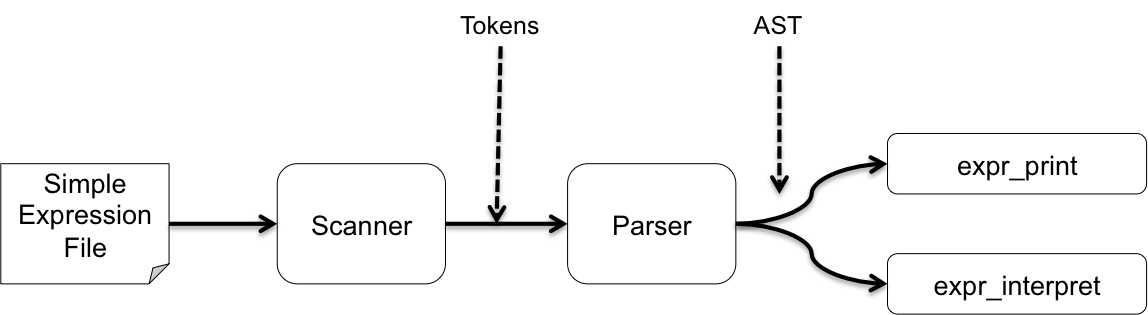
\includegraphics[width=0.75\columnwidth]{parser-diag} % Example image
\caption{Program Structure}
\label{parser-diag}
\end{center}
\end{figure}

\subsection{Files}
We provide a starter kit that will help guide you in your
implementation. Here is a brief description of the important files
contained in this project: \\

\begin{tabular}{l|p{10cm}}
  \textbf{File}          & \textbf{Description}                  \\
  \hline
  \hline
  Makefile               & A Makefile for building the parser    \\
  grammar.txt            & The grammar for expressions           \\
  src/expr-scanner.[h/c] & The scanner interface and 
                           implementation files for generating 
                           tokens from a simple expression 
                           contained in a file. \\
  src/expr-ast.[h/c]     & The AST interface and implementation 
                           files. It defines a data structure 
                           representation of the AST for simple 
                           expressions and prototypes for 
                           functions that operate over that AST structure. \\
  src/expr-parser.[h/c]  & The parser interface and implementation. 
                           It will use the scanner to read tokens 
                           and construct an AST. \\
  src/main.c             & The main entry point into the program \\
  expr-parser-soln       & The parser executable generated by our solution \\
  \hline
\end{tabular}

\subsection{Download \& Build}
First, download the starter kit and place it in your vagrant
folder. You will notice that this is a zip archive which you will need
to unzip using either \texttt{unzip} from the command line or some
other unzip program. Once you unzip the starter kit you will see the
\texttt{expr-parser-assignment} folder. Working from the terminal you
should \texttt{cd} into this folder. To compile the starter kit you
can execute the following command from the shell: \\

\begin{lstlisting}[frame=none]
vagrant> make
\end{lstlisting}

This will produce object files (.o) for each of the main components
and generate a final executable: \emph{expr-parser}. You can invoke
the program from the command line:

\begin{lstlisting}[frame=none]
usage: expr-parser FILE
\end{lstlisting}

To remove all the files created during compilation (e.g., .o,
expr-parser) you run this command:

\begin{lstlisting}[frame=none]
vagrant> make clean
\end{lstlisting}

This will remove both object files and the generated binary executable
files.

\subsection{Details}
The parser is structured into three important modules:
\textbf{scanner}, \textbf{ast}, and \textbf{parser} (as depicted in
Figure \ref{parser-diag}). In this assignment you should focus your
attention toward the ast and parser modules. You will also want to
look at \texttt{main.c} to get an understanding of how the program
begins executing and how it interacts with the components. You can see
what the output looks like by running our solution parser:

\begin{lstlisting}[frame=none]
vagrant> ./expr-parser-soln test/test_07.txt
expr = (((3+4)*(2+3))/(5*1))
7
\end{lstlisting}

As you can see it first prints out the AST that is constructed
followed by the result of evaluating the expression.

\subsection{Abstract Syntax Trees}
The AST interface is defined in the \texttt{expr-ast.h} header
file. It provides definitions of each of the important nodes found in
an abstract syntax tree for simple expressions: \texttt{Int},
\texttt{Term}, \texttt{Factor}, and \texttt{Expr}. The \texttt{Expr}
struct is used to represent an expression that can either be an
\emph{Int}, \emph{Term}, or \emph{Factor}. In C, we can accomplish
this by using a \emph{union} along with a type to indicate which
object the Expr object points to. The \texttt{expr\_type} enum does
exactly this by defining the symbolic constants \texttt{INT},
\texttt{TERM}, \texttt{FACTOR} (see Listing
\ref{../soln-src/expr-ast.h}). Thus, to create an expression that
represents a Term we would write the following C code:

\begin{lstlisting}[frame=none]
Expr e;
e.term = malloc(sizeof(Term));
e.t = TERM;
\end{lstlisting}

Why do we do this? In the days before object-oriented languages and
inheritance we still wanted to operate on values of different types -
yet belonging to the same category. In our case, we have Int, Factor,
and Term, all of which are an Expr, but have potentially different
implementations. In modern object-oriented languages we would simply
create a base class or interface called Expr and extend it with each
of the corresponding types (Int, Term, Factor). C accomplishes this
with the union and type identifier. \\

The AST module also provides prototype (interface) definitions for
creating each of the important expressions as well as the functions
for printing an expression and interpreting an expression:

\begin{lstlisting}[frame=none]
int expr_print(Expr* expr);
int expr_interpret(Expr* expr);
\end{lstlisting}

\texttt{expr\_print} takes an \texttt{Expr*} as its argument. It will
print the AST to \emph{stdout} in the same format as it was read in
from the text file. The only difference is that \texttt{expr\_print}
will also add a '(' and ')' around each expression in the AST. For
example, in \texttt{test/test\_02.txt} we have the expression:

\begin{lstlisting}[frame=none]
4*5+2*3+4*6*7;
\end{lstlisting}

\texttt{expr\_print} will produce the following to standard output:

\begin{lstlisting}[frame=none]
((4*5)+((2*3)+(4*(6*7))))
\end{lstlisting}

As you can see each of the sub-expressions have been wrapped in
parenthesis. This makes it clear that you are constructing the AST
properly. This function returns 1 if the expression was printed
successfully; 0 otherwise. \texttt{expr\_interpret} takes an
\texttt{Expr*} as its argument. It will evaluate the expression and
return the resulting value. Thus, it will recursively visit the nodes
in the AST evaluating each in turn. Note, that this is a bottom-up
process. We must first evaluate the leaves, then the internal nodes of
the tree. For example, given the simple expression 1*2+3*4 we would
have the AST: \\

\begin{figure}
\begin{center}
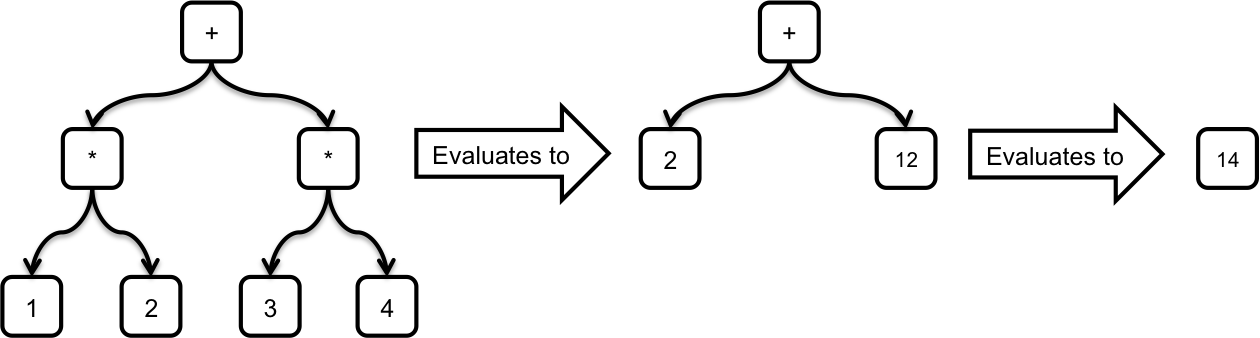
\includegraphics[width=0.75\columnwidth]{evaluate} % Example image
\caption{Evaluating a Tree}
\label{evaluate-diag}
\end{center}
\end{figure}

We would first need to evaluate the leaves - which are \texttt{Int}
nodes. This is easy because the Int nodes evaluate to themselves. We
then evaluate the '*' operators. We would then evaluate the '+'
operator. The process is illustrated in Figure \ref{evaluate-diag}. We
can define the rules of evaluation recursively as we do in the
following rules:

\begin{lstlisting}[frame=none]
expr_interpret(e) => return e.value, if e is an Int
expr_interpret(e) => return expr_interpret(e.left) + expr_interpret(e.right),
              if e is a term whose operator is +
expr_interpret(e) => return expr_interpret(e.left) - expr_interpret(e.right),
              if e is a term whose operator is -
expr_interpret(e) => return expr_interpret(e.left) * expr_interpret(e.right),
              if e is a factor whose operator is *
expr_interpret(e) => return expr_interpret(e.left) / expr_interpret(e.right),
              if e is a factor whose operator is /
expr_interpret(e) => print ``failure'' if e is NULL
\end{lstlisting}

\subsection{Parser}
You will need to complete the implementation of the parser. There are
four \emph{TODO} comments in the \texttt{parser.c} file that you will
need to replace with your implementation. The functions that you need
to implement are:

\begin{lstlisting}[frame=none]
Expr* parse_expr();
Expr* parse_expr_prime(Expr* left);
Expr* parse_term();
Expr* parse_term_prime(Expr* left);
\end{lstlisting}

We have provide the implementation of \texttt{expr\_parse(char*
  filename)} and \texttt{parse\_factor()}. Each function is described
in the comments and you should follow the grammar exactly. You should
note that two of the functions above take an expression as its
argument. This corresponds to the parsing of the expression on the
left-hand side of the possible operator. You will need to pass the
constructed Expr object from the calling parse function to it so you
can complete the construction of the AST. You should also note that
this parser implementation does take into account operator precedence,
however, it does not take into consideration the associativity of
operators. That is, given the expression 1*2*3*4*5*6*7*8*9
(\texttt{test/test\_08.txt}), the solution parser will generate the
following output:

\begin{lstlisting}[frame=none]
expr = (1*(2*(3*(4*(5*(6*(7*(8*9))))))))
362880
\end{lstlisting}

Although this constructs a reasonable AST and is evaluated properly it
does not encode the associativity of the * operator correctly in the
AST. The * operator is left-associative, however, the AST encodes this
as right-associative. For this assignment you need not worry about the
associativity of the operators. In your implementation you should use
the functions:

\begin{lstlisting}[frame=none]
int match(TOKEN_TYPE ttype);
int consume(TOKEN_TYPE ttype);
\end{lstlisting}

to match and consume tokens. The \texttt{match} function will return 1
if the current token from the scanner has the token type
\texttt{ttype}; 0 otherwise. The \texttt{consume} function will read
in the next token from the scanner if the current token matches the
token type \texttt{ttype}. This function returns 1 if successful; 0
otherwise. See the implementation of \texttt{parse\_factor} to see how
these functions are used.

\subsection{Tasks}
Your job is to complete the following:

\begin{itemize}
  \item Implement the \texttt{expr\_print} function in
    \texttt{expr-ast.c} (\textbf{25 points})
  \item Implement the \texttt{expr\_interpret} function in
    \texttt{expr-ast.c} (\textbf{25 Points})
  \item Complete the implementation of the parser. You should consult
    the \texttt{grammar.txt} file to see the grammar that the parser
    is using - the grammar is also noted in the comments in
    \texttt{expr\_parser.c}. You should not deviate from this grammar
    definition (\textbf{50 Points})
\end{itemize}

%Listing \ref{../soln-src/expr-parser.h} shows C code.
%\code{../soln-src/expr-parser.h}{Sample C Code!}
%\lipsum[1]

\subsection{Submission}
Please submit your assignment to Moodle by the assigned due date. You
should zip the entire assignment directory and submit to moodle. You
should make sure that you do a \texttt{make clean} before you submit
your assignment to reduce the size of your submission.

\subsection{Appendix A}

\code{../soln-src/expr-ast.h}{AST Header File}

\end{homeworkProblem}

%% %----------------------------------------------------------------------------------------
%% %	PROBLEM 2
%% %----------------------------------------------------------------------------------------

%% \begin{homeworkProblem}
%% \lipsum[2]

%% \problemAnswer{
%% \begin{center}
%% \includegraphics[width=0.75\columnwidth]{example_figure} % Example image
%% \end{center}

%% \lipsum[3-5]
%% }
%% \end{homeworkProblem}

%----------------------------------------------------------------------------------------

\end{document}
